\section{Benchmarking}
\label{sec:res_bench}
This section presents the result from the IOZone benchmarking tests run on each filesystem. The output result is divided into a table for each test for each filesystem. Each table presents the benchmark performance of the test for each file size and each buffer size. Each table has five rows and 13 columns, where each cell is the performance of the test with the specific file size and buffer size. The complete data tables and graphs presenting the performance of each file system for the different file sizes can be found in Appendix~\ref{app:bench_data}.

The IOZone benchmarking for \gls{FFS} ran for 41 minutes, and the IOZone benchmarking for \gls{GCSF} took 20 minutes. They were started at the same time and the internet speed tests ran every five minutes until the benchmarking of \gls{FFS} was completed. In total, eight speed tests were conducted with an average latency of \SI{15.22}{\milli\second}. The average download speed was \SI[per-mode = symbol]{90.96}{\mega\bit\per\second} and the average upload speed was \SI[per-mode = symbol]{92.95}{\mega\bit\per\second}.

Combining the 55 data points in one table, we get the overall performance of a test. Using this data, we can plot a box plot presenting the spread of the values in the table. Figure~\ref{fig:res_box_read} presents a box plot of the benchmarking results of the filesystems for the Read test. It can be observed that the read operation performance of \gls{FFS} and \gls{FFFS} are in general worse than the performance for \gls{GCSF} and \gls{APFS}. \gls{FFS} has by far the biggest spread of values, and \gls{FFFS} has also a significant spread. The median performance of \gls{FFS} and \gls{FFFS} are similar. \gls{GCSF} and \gls{APFS} have less spread. The median performance of \gls{GCSF} and \gls{APFS} are significantly higher than the median performance of \gls{FFS} and \gls{FFFS}, and \gls{APFS} has the highest read performance of the four filesystems.

\begin{figure}[!htb]
	\label{fig:res_box_read}
	\begin{center}
		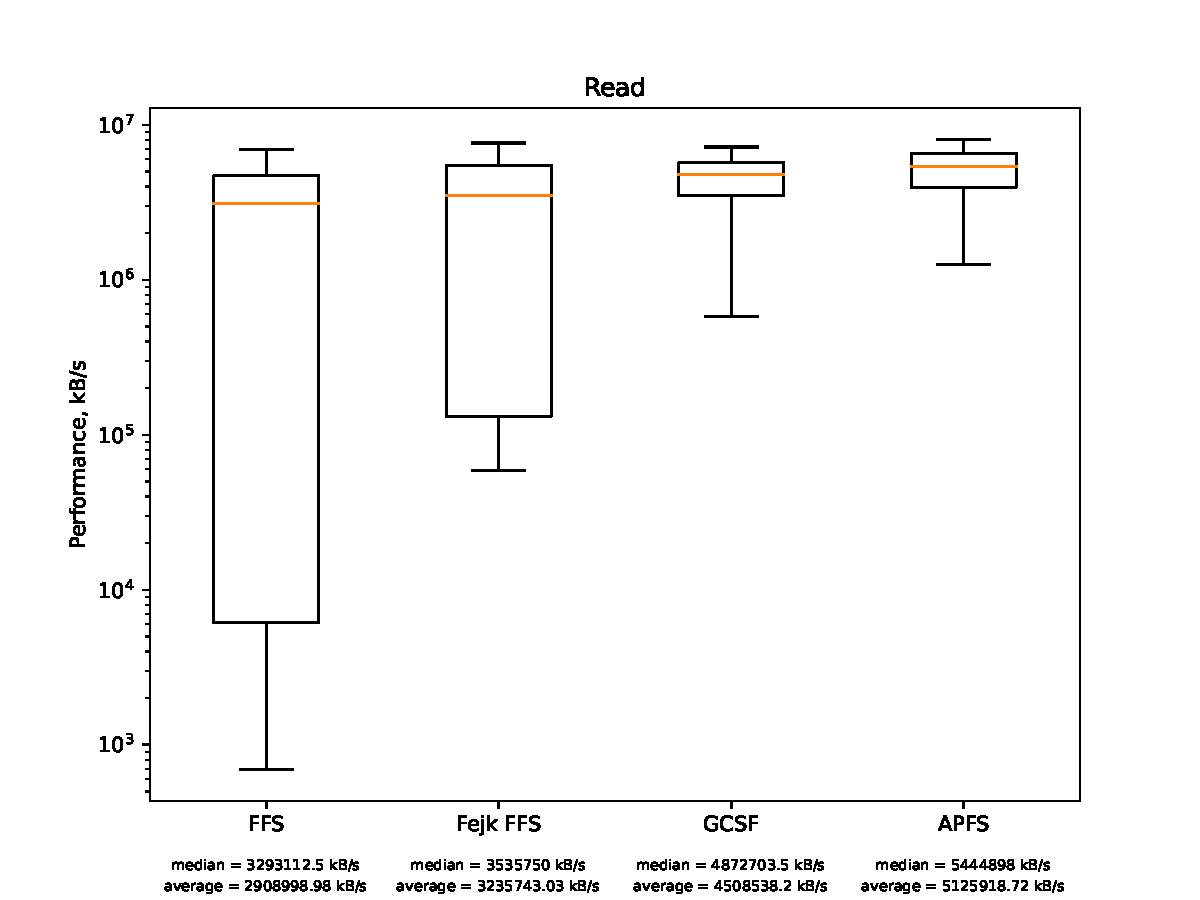
\includegraphics[width=1.0\textwidth]{figures/benchmarking/Read_box.pdf}
	\end{center}
	\caption{Box plot of the IOZone output for the Read test on the different filesystems}
\end{figure}

Figure~\ref{fig:res_box_write} presents a box plot of the benchmarking results of the filesystems of the Write test. \gls{APFS} has the best median write performance of the four filesystems, followed by \gls{FFFS}. The cloud-based filesystems \gls{FFS} and \gls{GCSF} have the worst median write performance, where \gls{FFS} has the worst performance of the filesystems. Comparing with the results of the Read test as presented in Figure~\ref{fig:res_box_read}, it can also be noted that the write performance is significantly worse for the write operations than the read operations for all filesystems. The average performance of the Write test for \gls{APFS} is 11\% of the Read performance. For \gls{FFFS}, \gls{GCSF}, and \gls{FFS} this percentage is 0.32\%, 0.05\%, and 0.02\%.

\begin{figure}[!htb]
	\label{fig:res_box_write}
	\begin{center}
		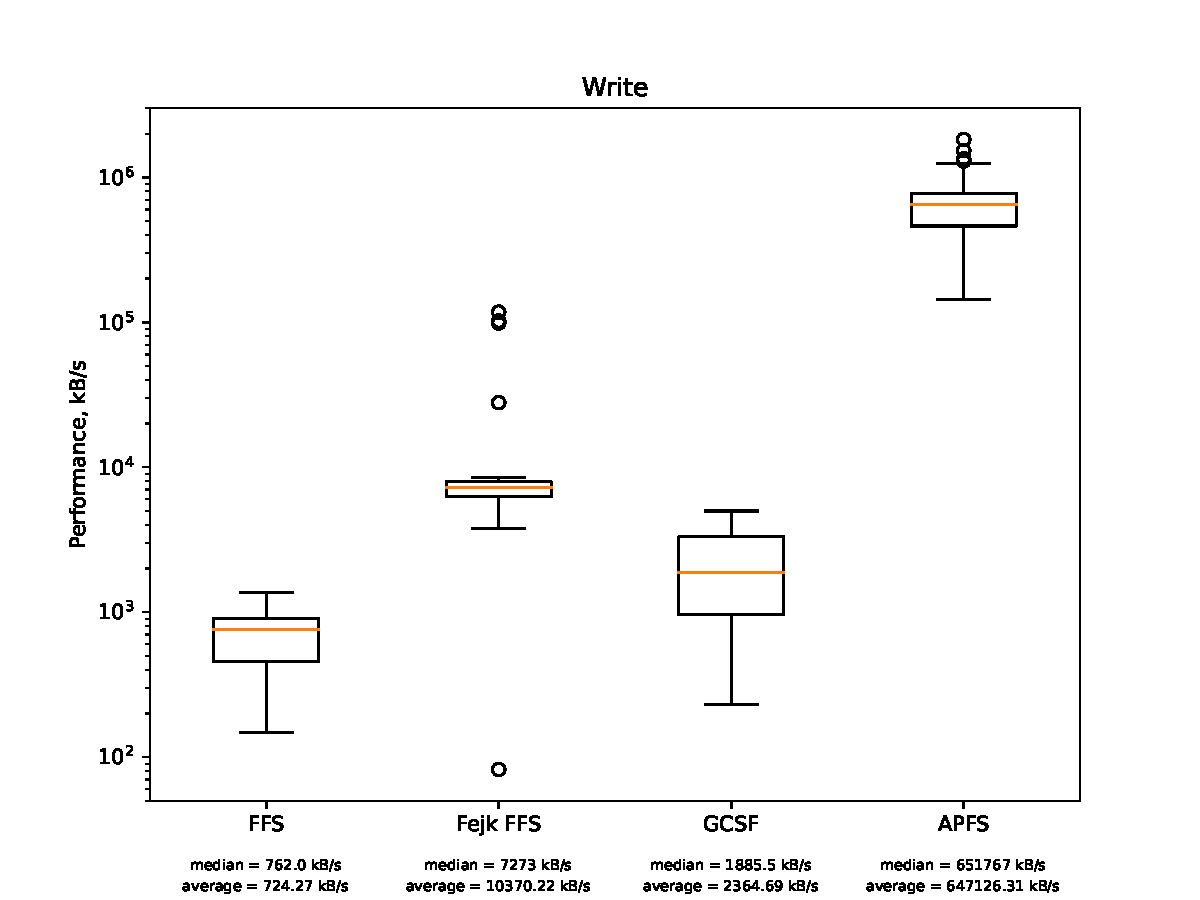
\includegraphics[width=1.0\textwidth]{figures/benchmarking/Write_box.pdf}
	\end{center}
	\caption{Box plot of the IOZone output for the Write test on the different filesystems}
\end{figure}

Figure~\ref{fig:res_box_reread} presents the result of the \mbox{Re-Read} test for the filesystems. The median performance of the filesystems are similar, with the performance of \gls{FFS} being lowest. Furthermore, the spread of the values for \gls{FFS} is greater than for the other filesystems. While the average performance for the Re-Read test of \gls{FFS} is around \SI[per-mode = symbol]{3}{\giga\byte\per\second}, the lowest performance was at \SI[per-mode = symbol]{468}{\kilo\byte\per\second}, namely for \texttt{file size = 1024, buffer size = 1024}. The spread of values is higher for \gls{APFS} than for \gls{FFFS} and \gls{GCSF}. The average and median performance of \gls{FFFS} and \gls{GCSF} are both higher than for \gls{APFS}. \gls{FFFS} has a higher average performance than \gls{GCSF}, while \gls{GCSF} has the highest median performance.

\begin{figure}[!htb]
	\label{fig:res_box_reread}
	\begin{center}
		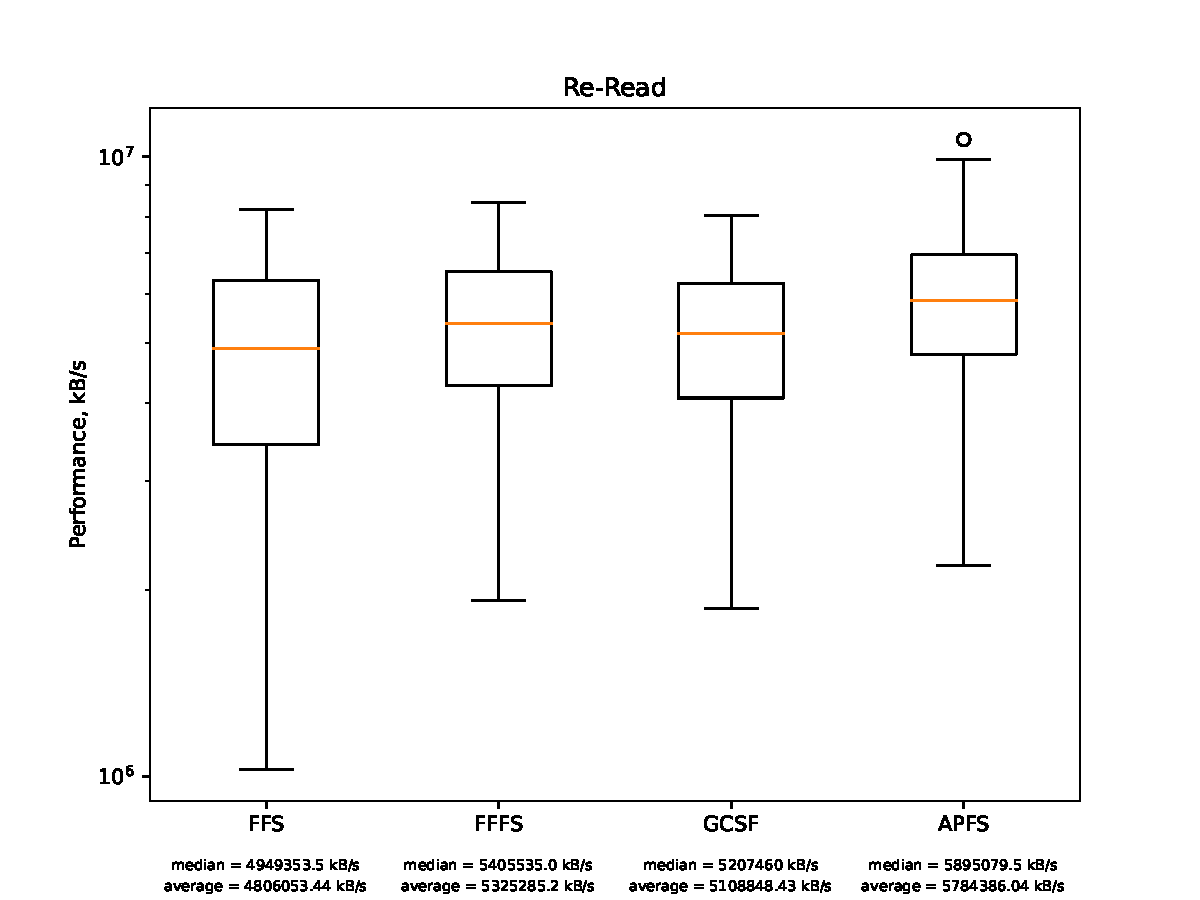
\includegraphics[width=1.0\textwidth]{figures/benchmarking/Re-Read_box.pdf}
	\end{center}
	\caption{Box plot of the IOZone output for the Re-Read test on the different filesystems}
\end{figure}

Figure~\ref{fig:res_box_rewrite} presents a box plot for the \mbox{Re-Write} test for the filesystems. Similar to the Write test results presented in Figure~\ref{fig:res_box_write}, \gls{APFS} has the best performance of the filesystems, followed by \gls{FFFS} and finally the two cloud-based filesystems. The performance of the filesystems are overall very similar to the results for the Write test. 

\begin{figure}[!htb]
	\label{fig:res_box_rewrite}
	\begin{center}
		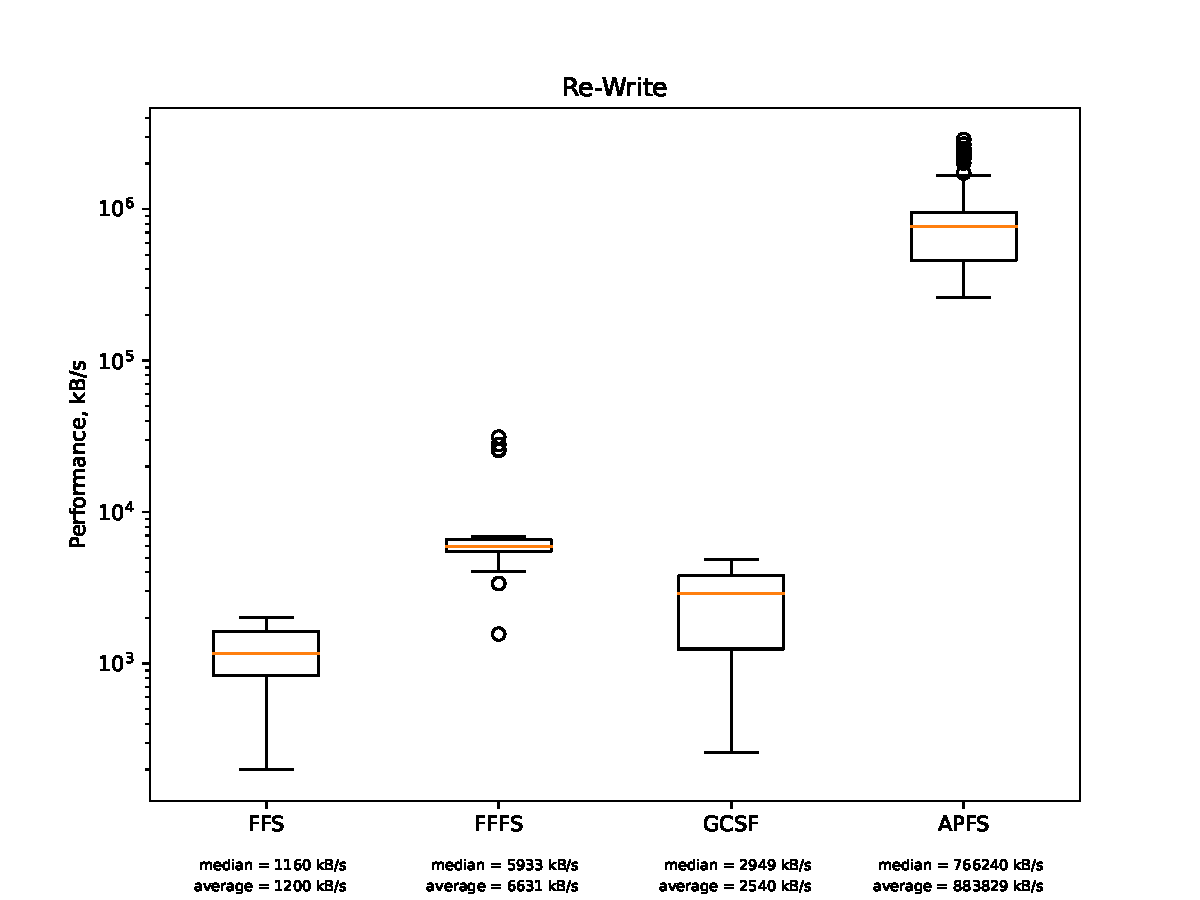
\includegraphics[width=1.0\textwidth]{figures/benchmarking/Re-Write_box.pdf}
	\end{center}
	\caption{Box plot of the IOZone output for the Re-Write test on the different filesystems}
\end{figure}

Figure~\ref{fig:res_box_rndread} presents a box plot for the Random read test for the different filesystems. The results are similar to the results for the \mbox{Re-Read} test presented in Figure~\ref{fig:res_box_reread}. \gls{FFFS} has the best average and median performance of the filesystems, and \gls{GCSF} has also better median and average performance than \gls{APFS}. The median and average performance of \gls{FFS} is lower than the other filesystems. \gls{FFS} also has a wide spread of values.

\begin{figure}[!htb]
	\label{fig:res_box_rndread}
	\begin{center}
		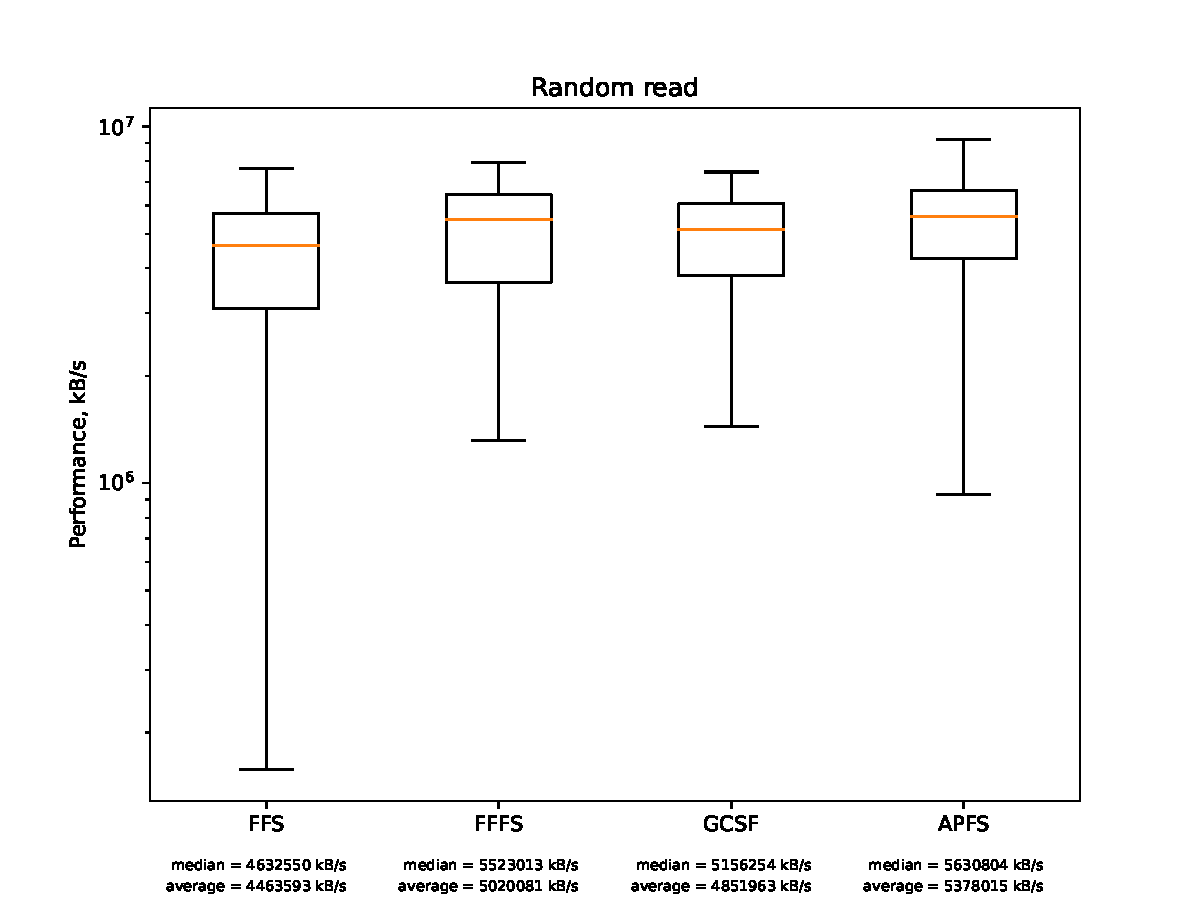
\includegraphics[width=1.0\textwidth]{figures/benchmarking/Random read_box.pdf}
	\end{center}
	\caption{Box plot of the IOZone output for the Random read test on the different filesystems}
\end{figure}

Figure~\ref{fig:res_box_rndwrite} presents a box plot for the Random read test for the different filesystems. \gls{APFS} has the highest performance, followed by \gls{FFFS} and the cloud-based filesystems. \gls{GCSF} has better performance than \gls{FFS}. The difference between the Random read test and the \mbox{Re-Read} test is small for all filesystems. \gls{FFS} does not have the best performance in any of the box plots presented. \gls{GCSF} has better performance than \gls{FFS} for all tests run with the benchmarking.

\begin{figure}[!htb]
	\label{fig:res_box_rndwrite}
	\begin{center}
		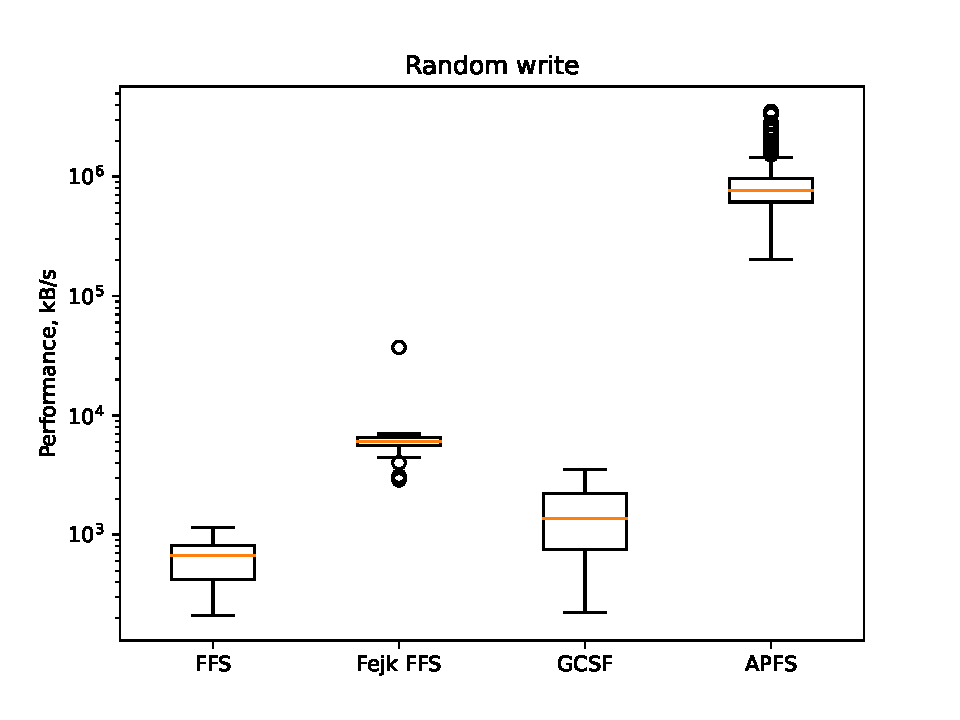
\includegraphics[width=1.0\textwidth]{figures/benchmarking/Random write_box.pdf}
	\end{center}
	\caption{Box plot of the IOZone output for the Random write test on the different filesystems}
\end{figure}

